\section{Grupos de procesos y áreas de conocimientos}

\subsection{Grupos de procesos de la dirección de proyectos}

\begin{enumerate}
    \item Inicialización: Autorización para comenzar dicho proyecto.
    
    \item Planeación: Establecer el alcance, refinar objetivos. 
    
    \item Ejecución: Procesos para completar el trabajo.
    
    \item Monitoreo y control: Regular desempeño del proyecto.
    
    \item Cierre: Todas las actividades para completar el trabajo.
\end{enumerate}

\begin{figure}[h!]
    \centering
        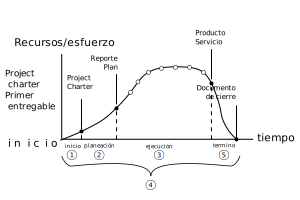
\includegraphics[scale=0.30]{Manufactura Integrada por Computadora Figuras/Figura02 Ciclo de Vida de Proyecto.png}
        \caption{Ciclo de vida de proyecto}
\end{figure}

\subsection{Áreas  de conocimiento}

\begin{enumerate}
    \item Gestión de la integración del proyecto: Tomar decisiones en cuanto a la asignación de recursos. Balancear objetivos y manejar las interdependencias entre áreas. 
    
    \item Gestión del alcance del proyecto: Definir y controlar lo que se incluye y lo que no.
    
    \item Gestión del tiempo del proyecto: Definir y secuenciar actividades, estimar recursos y duración de las actividades. 
    
    \item Gestión de los costos del proyecto: estimar, presupuestar y controlar los costos. 
    
    \item Gestión de la calidad del proyecto: Procesos y actividades para se satisfaga las necesidades. 
    
    \item Gestión de los recursos humanos del proyecto: Procesos que organizan, gestionan y conducen el proyecto. 
    
    \item Gestión de las comunicaciones del proyecto: Procesos que organizan, gestionan y conducen el proyecto.
    
    \item Gestión de riesgos del proyecto: Procesos para identificar, analizar, planear respuestas a los riesgos. 
    
    \item Gestión de las adquisiciones del proyecto: Procesos de compra de productos o servicios. administración de contratos y ordenes. 
    
    \item Gestión de los interesados del proyecto: Proceso para identificar personas, grupos que pueden afectar o ser afectados por el proyecto. 
\end{enumerate}

Linea base de un proyecto: Punto de medida de tiempo, alcance y recursos. 

\begin{figure}[h!]
    \centering
        \includegraphics[scale=0.30]{Manufactura Integrada por Computadora Figuras/Figura03 Triangulo de Hierro.png}
        \caption{Triangulo de hierro}
\end{figure}